%%%%%%%%%%%%%%%%%%%%%%%%%%%%%%%%%%%%%%%%%
% Beamer Presentation
% LaTeX Template
% Version 1.0 (10/11/12)
%
% This template has been downloaded from:
% http://www.LaTeXTemplates.com
%
% License:
% CC BY-NC-SA 3.0 (http://creativecommons.org/licenses/by-nc-sa/3.0/)
%
%%%%%%%%%%%%%%%%%%%%%%%%%%%%%%%%%%%%%%%%%

%----------------------------------------------------------------------------------------
%	PACKAGES AND THEMES
%----------------------------------------------------------------------------------------

\documentclass[aspectratio=169,usenames,dvipsnames]{beamer}

\usepackage[utf8]{inputenc}
\usepackage{booktabs}
\usepackage{tabularx}
\usepackage[authordate,bibencoding=auto,strict,backend=biber,natbib]{biblatex-chicago}
\addbibresource{bib.bib}
\usepackage{graphicx}
% \hypersetup{
%     colorlinks,
%     %citecolor=black,
%     linkcolor=black
% }
\usepackage{array}
\usepackage{caption}
\usepackage{threeparttable}
\usepackage{epigraph} 
\usepackage{lscape}
\usepackage{adjustbox}
\newcommand*{\Scale}[2][4]{\scalebox{#1}{\ensuremath{#2}}}%
\usepackage{import}
\newenvironment{wideitemize}{\itemize\addtolength{\itemsep}{10pt}}{\enditemize}
\usepackage{amsmath}
\usepackage{csvsimple}
\usepackage{siunitx}
\usepackage{filecontents}
\usepackage{rotating}
\usepackage{multirow}
\usepackage{amsmath}
\usepackage{subcaption}
\usepackage{appendixnumberbeamer}
\usepackage{float}
\usepackage{amsmath}
\usepackage{csvsimple}
\usepackage{hyperref}
\newtheorem{proposition}{Proposition}
\usepackage{xcolor}
\def\boxit#1#2{%
    \smash{\color{red}\fboxrule=1pt\relax\fboxsep=2pt\relax%
    \llap{\rlap{\fbox{\phantom{\rule{#1}{#2}}}}~}}\ignorespaces
}
\newenvironment{variableblock}[3]{%
  \setbeamercolor{block body}{#2}
  \setbeamercolor{block title}{#3}
  \begin{block}{#1}}{\end{block}}
\usepackage{appendixnumberbeamer}
\usepackage{tikz,pgfplots}
\usepackage{tkz-fct}
\usepackage{amsthm}
\pgfplotsset{compat=1.10}
\usepgfplotslibrary{fillbetween}
\mode<presentation> {
\AtBeginSection[]
{
    \begin{frame}
        \frametitle{Table of Contents}
        \tableofcontents[currentsection]
    \end{frame}
}
% The Beamer class comes with a number of default slide themes
% which change the colors and layouts of slides. Below this is a list
% of all the themes, uncomment each in turn to see what they look like.

\usetheme{default}
%\usetheme{AnnArbor}
%\usetheme{Antibes} -
%\usetheme{Bergen}
%\usetheme{Berkeley}
%\usetheme{Berlin}
%\usetheme{Boadilla}
%\usetheme{CambridgeUS}
%\usetheme{Copenhagen} -
%\usetheme{Darmstadt}
%\usetheme{Dresden}
%\usetheme{Frankfurt}
%\usetheme{Goettingen}
%\usetheme{Hannover}
%\usetheme{Ilmenau}
%\usetheme{JuanLesPins}
%\usetheme{Luebeck}
%\usetheme{Madrid}
%\usetheme{Malmoe}
%\usetheme{Marburg}
%\usetheme{Montpellier}
%\usetheme{PaloAlto}
%\usetheme{Pittsburgh}
%\usetheme{Rochester} -
%\usetheme{Singapore}
%\usetheme{Szeged}
%\usetheme{Warsaw}

% As well as themes, the Beamer class has a number of color themes
% for any slide theme. Uncomment each of these in turn to see how it
% changes the colors of your current slide theme.

%\usecolortheme{albatross}
%\usecolortheme{beaver}
%\usecolortheme{beetle}
%\usecolortheme{crane}
%\usecolortheme{dolphin}
%\usecolortheme{dove}
%\usecolortheme{fly}
%\usecolortheme{lily}
%\usecolortheme{orchid}
%\usecolortheme{rose}
%\usecolortheme{seagull}
%\usecolortheme{seahorse}
%\usecolortheme{whale}
%\usecolortheme{wolverine}

%\setbeamertemplate{footline} % To remove the footer line in all slides uncomment this line
%\setbeamertemplate{footline}[frame number] % To replace the footer line in all slides with a simple slide count uncomment this line
\setbeamertemplate{theorems}[numbered]
\setbeamertemplate{navigation symbols}{} % To remove the navigation symbols from the bottom of all slides uncomment this line
}
\setbeamertemplate{caption}{\raggedright\insertcaption\par}
  \setbeamertemplate{enumerate items}[default]
  %\setbeamertemplate{page number in head/foot}{\insertframenumber}
\usepackage{graphicx} % Allows including images
\usepackage{booktabs} % Allows the use of \toprule, \midrule and \bottomrule in tables
%\usepackage {tikz}
\newtheorem*{theorem*}{Theorem}
\newtheorem*{lemma*}{Lemma}
\newtheorem*{proposition*}{Proposition}
\newtheorem*{corollary*}{Corollary}
\newtheorem*{definition*}{Definition}
\DeclareMathOperator*{\argmin}{arg\,min}
\newtheorem*{assumption}{Assumption}
\usetikzlibrary {positioning}
\renewcommand{\arraystretch}{1.5}
\newcommand\hideit[1]{%
  \only<0| handout:1>{\mbox{}}%
  \invisible<0| handout:1>{#1}}
\usepackage[default]{lato}

\setbeamercolor{block body alerted}{bg=alerted text.fg!10}
\setbeamercolor{block title alerted}{bg=alerted text.fg!20}
\setbeamercolor{block body}{bg=structure!10}
\setbeamercolor{block title}{bg=structure!20}
\setbeamercolor{block body example}{bg=green!10}
\setbeamercolor{block title example}{bg=green!20}


\makeatletter
\let\save@measuring@true\measuring@true
\def\measuring@true{%
  \save@measuring@true
  \def\beamer@sortzero##1{\beamer@ifnextcharospec{\beamer@sortzeroread{##1}}{}}%
  \def\beamer@sortzeroread##1<##2>{}%
  \def\beamer@finalnospec{}%
}
\makeatother
%\usepackage {xcolor}

%----------------------------------------------------------------------------------------
%	TITLE PAGE
%----------------------------------------------------------------------------------------

\title[diss]{Lecture 5: The Risk-Incentive Trade-Off} % The short title appears at the bottom of every slide, the full title is only on the title page
\author{Compensation in Organizations} % Your name
\institute[shortinst]{Jacob Kohlhepp}
\date{\today} % Date, can be changed to a custom date

\begin{document}

\begin{frame}
\titlepage % Print the title page as the first slide

\end{frame}


\begin{frame}{Recalling Performance Pay Results}

\begin{theorem}
        When wages depend only on output, effort is $e_{p}$ which solves 
        \[c'(e_{p})= \frac{1}{1+r \sigma^2 c''(e_{p})}\]
        and $\beta_{p} =c'(e_{p}),\alpha_{p} =\bar u - \beta_{p} e_{p}+r \beta^2\sigma^2/2+c(e_{p})$.
    \end{theorem}
    \begin{wideitemize}
        \item Focus on: $c'(e_{p})= \frac{1}{1+r \sigma^2 c''(e_{p})}$
        \item As $\sigma^2$ rises, $\beta_p$ falls
        \item Incentives/performance pay/bonuses decrease with noise/luck/randomness.
        \item This is the risk-incentive trade-off.
        \item $e_p$ also generally falls, although this is harder to prove.
    \end{wideitemize}
    
\end{frame}


% \begin{frame}{Effort-Based Pay}
% \begin{theorem}
%         When wages depend directly on effort, effort is $e^*$ which solves $c'(e^*)=1$ and $\beta^*=1, \alpha^*=\bar u+c(e^*)-1$
%     \end{theorem}

%     \begin{wideitemize}
%         \item Question: how does $r$ impact outcomes under effort-based pay?
%         \pause
%         \item Question: Why does it have no impact?
%     \end{wideitemize}
% \end{frame}

% \begin{frame}{Performance-Based Pay}
%     \begin{theorem}
%         When wages depend only on output, effort is $e_{p}$ which solves 
%         \[c'(e_{p})= \frac{1}{1+r \sigma^2 c''(e_{p})}\]
%         and $\beta_{p} =c'(e_{p}),\alpha_{p} =\bar u - \beta_{p} e_{p}+r \beta^2\sigma^2/2+c(e_{p})$.
%     \end{theorem}

%     \begin{wideitemize}
%         \item Question: How does $r$ impact outcomes under performance-based pay?
%         \pause
%         \item Question: Why does it have this impact?
%     \end{wideitemize}
% \end{frame}

\begin{frame}{Trade-Off is (in some sense) Theoretically Robust}
\begin{wideitemize}
    \item The model we solved is a very special type of principal-agent model.
    \item We could allow for nonlinear wages, general output, etc.
    \item However, even when we do this, we still find that risk aversion reduces incentives and effort.
\end{wideitemize}
    
\end{frame}

\begin{frame}{Profit}

\begin{wideitemize}
    \item The level of effort is tied to total surplus/efficiency.
    \item As effort rises and goes to $e^*$, total surplus/efficiency rises.
    \item Therefore, since $e_p$ falls with $\sigma^2$, profit should fall.
    \item To see this very clearly, let's derive profit when $c(e)=e^2/2$.
    \item Remember: $e_p=\beta_p=\frac{1}{1+r \sigma^2}$ in this case!
\end{wideitemize}

\end{frame}

\begin{frame}{Profit Under Performance Pay and $c(e)=e^2/2$}

    \begin{align*}
        \pi_p &= e_p-c(e_p)-\frac{r\beta^2_p \sigma^2}{2}-\bar u\\
        &= \frac{1}{1+r \sigma^2} - \frac{1}{2(1+r \sigma^2)} - r\sigma^2\frac{1}{2(1+r \sigma^2)} -\bar u\\
        &= \frac{1}{1+r \sigma^2} \bigg ( 1- \frac{1}{2(1+r \sigma^2)}-r\sigma^2\frac{1}{2(1+r \sigma^2)}-\bar u\\
        &= \frac{1}{1+r \sigma^2} \bigg ( 1- \frac{1+r\sigma^2}{2(1+r \sigma^2)} \bigg )-\bar u\\
        &=\frac{1}{1+r \sigma^2} \bigg ( \frac{2(1+r \sigma^2)}{2(1+r \sigma^2)}- \frac{1+r\sigma^2}{2(1+r \sigma^2)} \bigg )-\bar u\\
        &=\frac{1}{1+r \sigma^2} \bigg (  \frac{1+r\sigma^2}{2(1+r \sigma^2)} \bigg )-\bar u\\
        &=\frac{1}{2}\frac{1}{1+r \sigma^2}-\bar u
    \end{align*}
    
    
\end{frame}


\begin{frame}{Performance Pay vs. Some Alternative Method}

\begin{wideitemize}
    \item Suppose the firm can use performance pay or some alternative with profit $\pi_{alt}$.
    \item It will choose performance paif if:
    \[\pi_p = \frac{1}{2}\frac{1}{1+r \sigma^2}-\bar u \geq \pi_{alt}\]
    \item As $\sigma^2$ rises, performance pay becomes less likely.
    \item This is a testable implication of the risk-incentive trade-off.
\end{wideitemize}
\end{frame}



\section{Evidence for the Risk-Incentive Trade-Off}

\begin{frame}{``Moral hazard and risk spreading in partnerships" (Gaynor and Gertler 1995)}
    \huge Discussion
\end{frame}


\begin{frame}{``Moral hazard and risk spreading in partnerships" (Gaynor and Gertler 1995)}
    \begin{wideitemize}
        \item Setting is medical group practices.
        \item At time of article, 61\% of physicians worked in group settings.
        \item In these groups, physicians are co-owners making decisions together, including fees and resource allocations.
        \item Physicians have specialties but demand can be highly variable across specialties (exmaple?)
        \item Data shows how much compensation depends on output (1-10), size of group, price of an office visit, and a measure of physician risk aversion.
    \end{wideitemize}
\end{frame}


\begin{frame}{``Moral hazard and risk spreading in partnerships" (Gaynor and Gertler 1995)}
    \begin{wideitemize}
        \item Concern: self-reported measure of risk aversion may just reflect what physician experiences rather than what they ``want."
        \item Alleviated: risk aversion measure is negatively correlated with performance pay measure.
        \item 10\% increase in incentives leads to 3.5\% more visits.
        \item Price decreases demand (why is this a good sign?)
    \end{wideitemize}
\end{frame}


\begin{frame}{``Moral hazard and risk spreading in partnerships" (Gaynor and Gertler 1995)}
    \begin{wideitemize}
        \item Varying risk aversion variable across full range alters ofice visits by over 877 per year.
        \item The most risk averse physicians make about \$11,582 less than the least risk averse.
        \item This is 10\% of mean income.
        \item It is a measure of the efficiency loss of partnerships.
    \end{wideitemize}
\end{frame}



\begin{frame}[c]{``Moral hazard and risk spreading in partnerships" (Gaynor and Gertler 1995)}
\centering
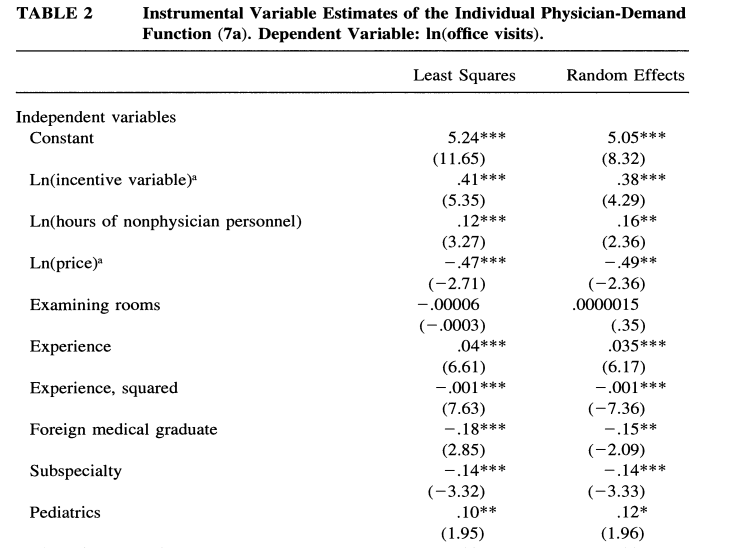
\includegraphics[width=0.7\textwidth]{pictures/demand_physicians.png}
\end{frame}

\begin{frame}[c]{``Moral hazard and risk spreading in partnerships" (Gaynor and Gertler 1995)}
\centering
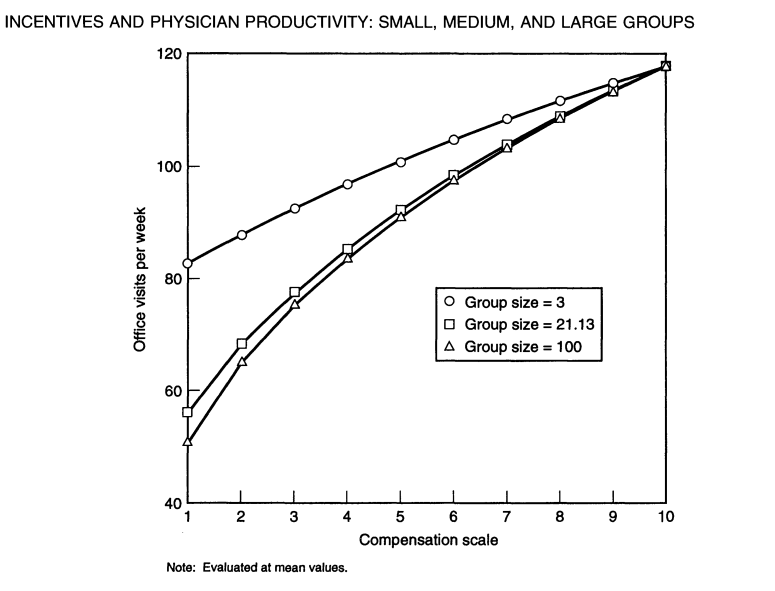
\includegraphics[width=0.7\textwidth]{pictures/physicians_comp_demand.png}
\end{frame}
\begin{frame}{``Moral hazard and risk spreading in partnerships" (Gaynor and Gertler 1995)}
\centering
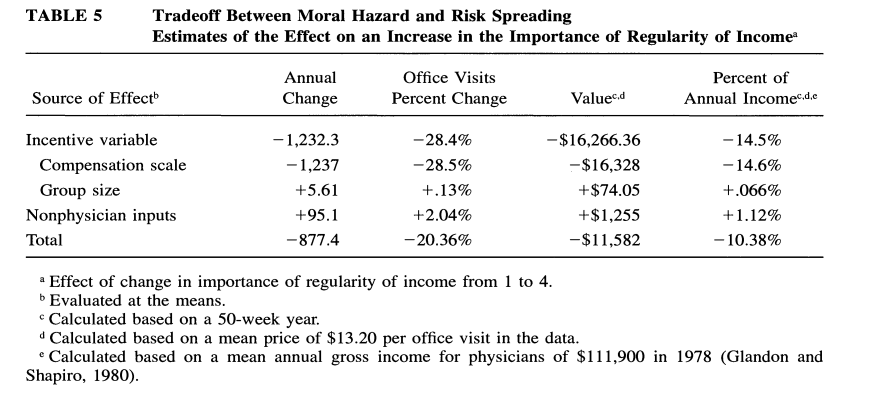
\includegraphics[width=0.9\textwidth]{pictures/physicians_riskspreading.png}
\end{frame}


\begin{frame}{``Is a Higher Calling Enough? Incentive Compensation in the Church" (Hartzell, Parsons, Yermack 2010)}

\begin{wideitemize}
    \item Recall the setting: Methodist ministers whoa re rotated but have their pay set by their congregation.
    \item The paper shows evidence that Methodist ministers pay is consistent with pay for performance.
    \item Ministers get more pay for adding more people to their church.
    \item Let's focus on the portions related to the risk-incentive trade-off.
\end{wideitemize}
\end{frame}

\begin{frame}{``Is a Higher Calling Enough? Incentive Compensation in the Church" (Hartzell, Parsons, Yermack 2010)}

\begin{wideitemize}
    \item The paper actually tests the risk-incentive trade-off two ways:
    \begin{wideitemize}
        \item By estimating how volatile each church location's membership is over 43 years.
        \item By comparing oil-driven locations vs. non-oil drivne locations
    \end{wideitemize}
    \item Both methods have problems (they are not the core result of the paper).
    \item But both point towards the existence of the risk-incentive trade-off.
\end{wideitemize}
\end{frame}

\begin{frame}{Hartzell, Parsons, Yermack 2010: Direct Computation of Volatility}

\begin{wideitemize}
    \item Idea: use the entire time series of 43 years to compute the standard deviation of membership changes.
    \item In our performance pay model, this is a proxy for $\sigma^2$ if we assume that effort does not change much over time.
    \item The authors classify a church as ``High Volatility" if the church's standard deviation is above the median.
    \item ``High Volatility" churches pay on average \$10.75 less per new member than the rest.
    \item This is 50\% less ``bonus" ($\beta$)
    \item One issue: perhaps at volatile churches the value of a member is just less (the coefficient on $e$ is smaller) so they use lower incentives.    
\end{wideitemize}
\end{frame}




\begin{frame}[c]{Hartzell, Parsons, Yermack 2010: Oil Booms}
\centering
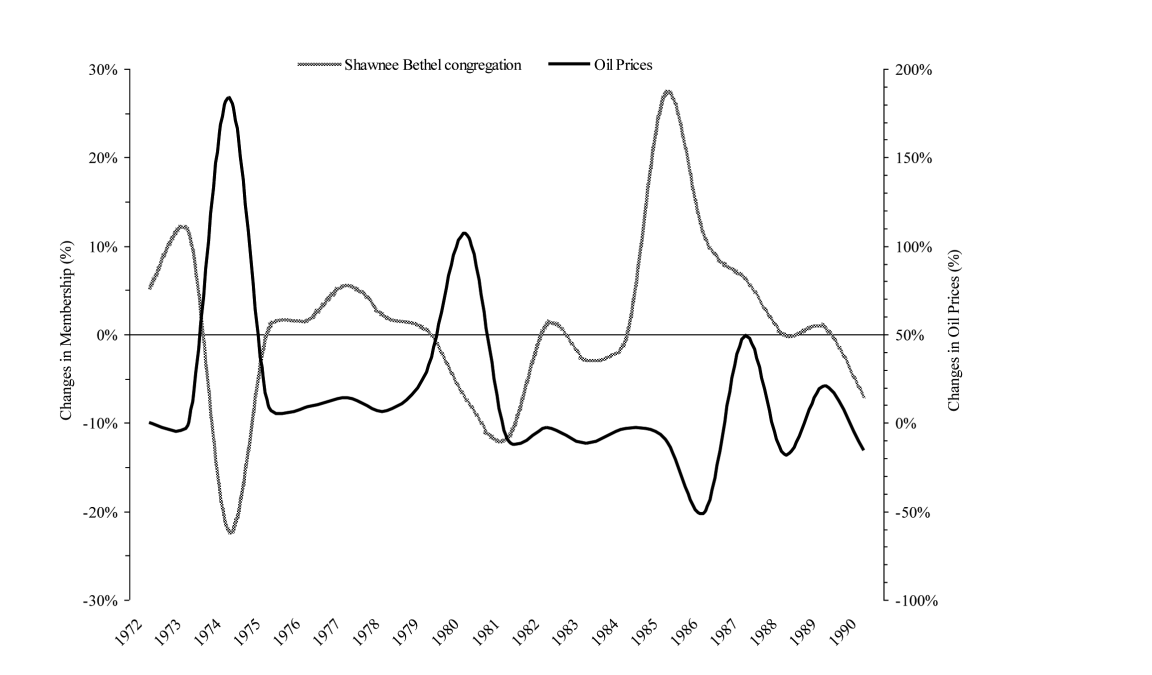
\includegraphics[width=0.9\textwidth]{pictures/oilboom.png}
\end{frame}


\begin{frame}{Hartzell, Parsons, Yermack 2010: Oil Booms}
\begin{wideitemize}
    \item Idea: use oil booms as proxy for volatility.
    \item This is ``better" because oil booms are an exogenous or external factor impacting attendance.
    \item Boom and bust clearly bring people in and out (direct cyclical effect).
    \item But also, as a town gets richer from oil, attendance may also drop.
\end{wideitemize}
\end{frame}


\begin{frame}[c]{Hartzell, Parsons, Yermack 2010: Results}
\centering
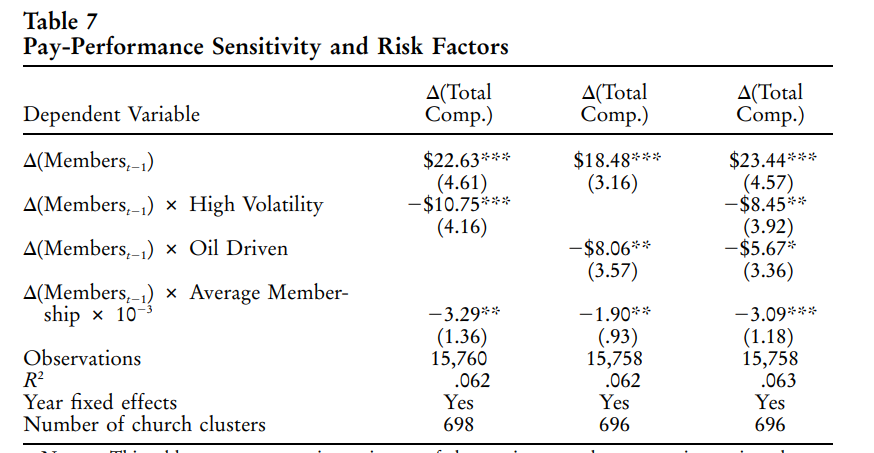
\includegraphics[width=0.9\textwidth]{pictures/oil_paytable.png}
\end{frame}


\section{Evidence Against the Risk-Incentive Trade-Off}


\begin{frame}[c]{``The Tenous Trade-off Between Risk and Incentives" (Prendergast 2002)}
\centering
    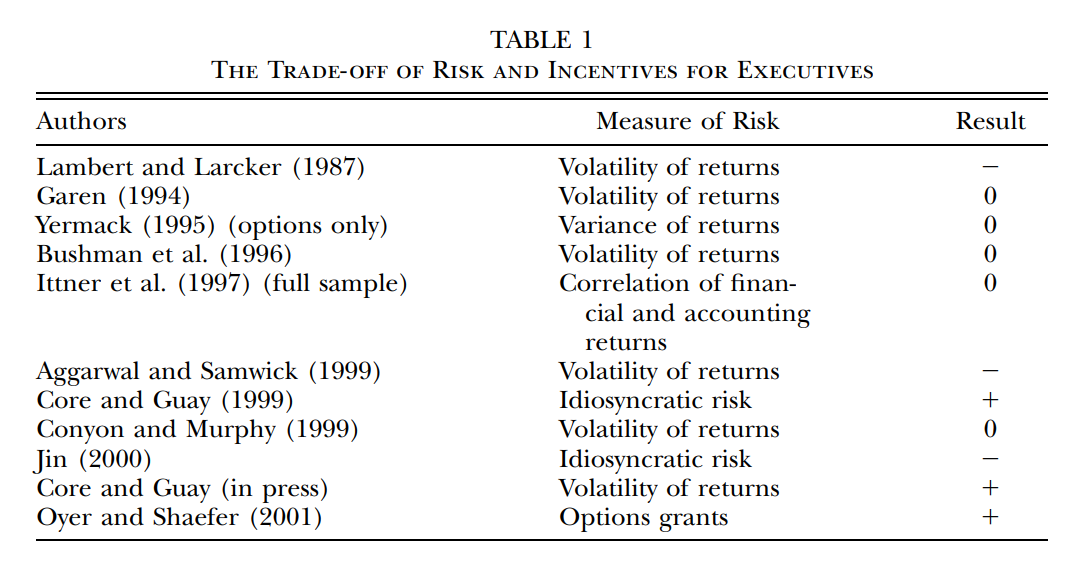
\includegraphics[width=0.9\textwidth]{pictures/ceos_tenous.png}
\end{frame}


\begin{frame}[c]{``The Tenous Trade-off Between Risk and Incentives" (Prendergast 2002)}
The amount sharecroppers keep ($\beta$) is positively associated with noise ($\sigma^2$).
\centering
    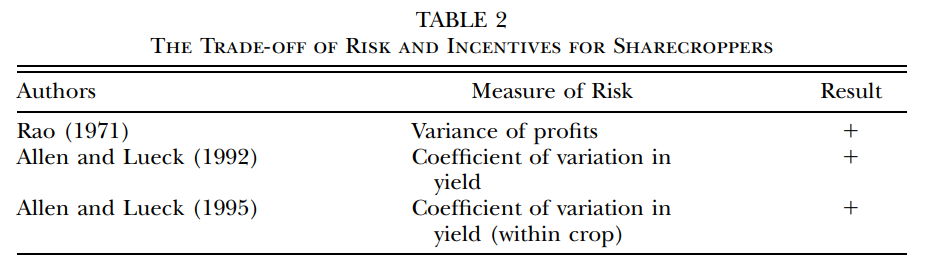
\includegraphics[width=0.9\textwidth]{pictures/sharecroppers.png}
\end{frame}

\begin{frame}[c]{``Incentive Contracting and the Franchise Design.” (Lafontaine and Slade (2001))}
\centering
    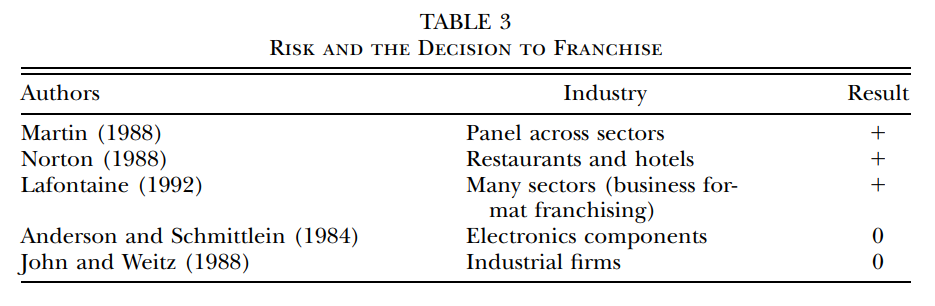
\includegraphics[width=0.9\textwidth]{pictures/franchise_risk.png}
\end{frame}

\section{(Potential) Resolutions of the Controversy}


\begin{frame}{Choosing What to Do}

\begin{wideitemize}
    \item Our model assumes the worker only chooses $e$.
    \item But what if the worker also chooses what to exert effort on.
    \item For this discussion assume the firm can measure effort.
    \item What if also the worker knows the benefit of each activity, but the firm does not?
\end{wideitemize}



\small Supporting source: ``The Tenous Trade-off Between Risk and Incentives" (Prendergast 2002)

    
\end{frame}


\begin{frame}{Choosing What to Do}

\begin{wideitemize}
    \item The firm has two choices: (1) choose what the agent can do and specify an effort based wage (2) let the agent choose and specify and output based wage.
    \item We can get the right effort from (1), but the firm might choose the wrong  activity.
    \item We will get the wrong effort from (2) but the worker will choose the right activity (why?)
    \item The key observation is that the maximum of random variables generally depends on variance.
\end{wideitemize}

\small Supporting source: ``The Tenous Trade-off Between Risk and Incentives" (Prendergast 2002)

    
\end{frame}


\begin{frame}{Choosing What to Do}

\begin{wideitemize}
     \item For two normal random variables with mean 0 and variance $\sigma^2$ we have:
    \[E[\max\{\epsilon_1, \epsilon_2\}]=\frac{\sigma}{\pi} \]
    \item So ``delegation" using performance pay $w(y)$ (option 1) becomes better relative to effort-based pay and command and control (option 2) when variance is larger.
    \item This overturns our earlier result and suggests a positive relationship between risks and performance pay!
    \item CEOs, franchising, etc. requires making complex decisions with situation-specific knowledge.
\end{wideitemize}



\small Supporting source: ``The Tenous Trade-off Between Risk and Incentives" (Prendergast 2002)

    
\end{frame}

\begin{frame}{Favoritism in Performance Evaluations}

\begin{wideitemize}
     \item If a supervisor likes a subordinate, it is costly to give them a bad performance evaluation.
     \item And this cost is larger when more is on the line (think about if the evaluation costs the person their job)
     \item Therefore stronger incentives make supervisors less truthful about employee performance.
     \item Firms might care about evaluations not just to induce effort but also to assign the employee to the right tasks.
\end{wideitemize}



\small Source ``Uncertainty and Incentives" (Prendergast 2002)

    
\end{frame}


\begin{frame}{Favoritism in Performance Evaluations}

\begin{wideitemize}
     \item In this context, we can think of risk as the supervisor knowing less about the employee's performance
     \item So their evaluation is noisy and not useful for assigning the worker to tasks.
     \item So the firm uses more performance pay because the ``sorting distortion" is low.
     \item This causes a positive link betwene incentives and risk!
\end{wideitemize}



\small Source ``Uncertainty and Incentives" (Prendergast 2002)

    
\end{frame}



\begin{frame}{Deciding When to Investigate}

\begin{wideitemize}
     \item In our model, we assumed output is always known.
     \item In reality, output is only sometimes monitored.
     \item Further, it is monitored more often when people suspect slacking/shirking/cheating.
     \item Consider a model where a supervisors chooses whether to launch an investigation.
     \item If no investigation, the worker gets a wage equal to expected output (so a flat salary)
     \item If investigated, they get actual output.
\end{wideitemize}



\small Source ``Uncertainty and Incentives" (Prendergast 2002)

    
\end{frame}


\begin{frame}{Deciding When to Investigate}

\begin{wideitemize}
     \item When deciding to investigate, the supervisor gets a signal or impression of output.
     \item There is some cost to investigation (laying it out here is beyond the scope of this class)
     \item The supervisor investigates if the expected benefit of doing so is great enough.
     \item In this setting, greater performance pay ($\beta$) is needed to encourage effort when noise is greater, because we also need to encourage investigations.
     \item Intuitively, noise makes workers think they can get away with it.
     \item this also generates a positive link between risk and incentives.
\end{wideitemize}



\small Source ``Uncertainty and Incentives" (Prendergast 2002)

    
\end{frame}


% https://www.journals.uchicago.edu/doi/full/10.1086/341874

% https://www.journals.uchicago.edu/doi/full/10.1086/338676

% https://pubs.aeaweb.org/doi/pdf/10.1257/aer.90.2.421


% \section{(Potential) Resolutions of the Controversy}


% \begin{frame}{Command and Control}    
% \begin{wideitemize}
%     \item What can a firm do instead of performance pay to encourage a worker?
%     \pause
%     \item Tell the worker exactly what to do, and monitor them to make sure they do it.
%     \item This itself does not go against the risk-incentive trade-off.
%     \item However, command and control only works if the firm knows what the agent should be doing.
%     \item In other words, the main alternative to performance pay works best when there is little uncertainty.
%     \item This implies we should expect MORE performance pay in uncertain settings.
% \end{wideitemize}
% \end{frame}

% \begin{frame}{Choosing to Investigate}

% \begin{wideitemize}
%     \item We assumed that performance/output is always monitored by the firm.
%     \item In reality, monitoring is less frequent and usually triggered by something.
%     \item Suppose the firm sometimes knows nothing about $y$ and sometimes gets some ``signal" or impression or ``vibe" about $y$.
%     \item Importantly vibes or signals or impressions are not contractible or verifiable, so the firm cannot use them to write a compensation contract.
%     \item The firm can decide to investigate using the signal, and use the results of the investigation to alter pay.
% \end{wideitemize}
    
% \end{frame}


% \begin{frame}{Choosing to Investigate}

% \begin{wideitemize}
%     \item In more uncertain environments (higher $\sigma^2$) the worker knows they can get away with more.
%     \item So the agent 
% \end{wideitemize}
    
% \end{frame}


%  \begin{frame}{Biased Performance Evaluations}
% https://www.journals.uchicago.edu/doi/abs/10.1086/338676?casa_token=B3qWZ0JxOjEAAAAA%3ADG6U2QppgBTwOuK-1PtHU6vVUdlIzpxPekyAxv5FvjcMNJM8ik-rbM3hL8XADpPRpKoIep3mUX8&journalCode=jole
%  \begin{wideitemize}
    
% \end{wideitemize}
    
% \end{frame}


%  \begin{frame}{Bunched Performance Evaluations}
% https://www.journals.uchicago.edu/doi/abs/10.1086/338676?casa_token=B3qWZ0JxOjEAAAAA%3ADG6U2QppgBTwOuK-1PtHU6vVUdlIzpxPekyAxv5FvjcMNJM8ik-rbM3hL8XADpPRpKoIep3mUX8&journalCode=jole
%  \begin{wideitemize}
    
% \end{wideitemize}
    
% \end{frame}






\end{document}







